\documentclass[12pt]{article}
\usepackage{amsmath}
\usepackage[english]{babel}
\usepackage{graphicx}
\usepackage{subfig}
\usepackage{amssymb}

\usepackage{hyperref}
\hypersetup{
    colorlinks=true,
    linkcolor=blue,
    filecolor=magenta,      
    urlcolor=cyan,
}

\title{Detecting House Numbers in Street View Imagery using Convolutional Neural Networks}
\author{Matthew Peyrard}
\date{\today}

\begin{document}
\maketitle

\section{Definition}
\subsection{Project Overview}
Fully automated GPS and mapping services have become an indespensible part of our daily lives.
Keeping such services up to date is a very large task with a lot of available room for automation.
Cataloging house numbers from street view imagery is an important part of the mapping process.
The process of manually identifying and cataloging such imagery is very expensive due to the scale at which such a process must be applied.
However, if computational resources could be applied to the task with reasonably high accuracy, then the process could be sped up enormously, in addition to the costs saved from not having to hire thousands of people to perform the task manually.

In this project, I created a machine learning application that is capable of reading batches of images of street view house numbers, and outputting what numbers they are in a computer readable format.

\subsection{Problem Statement}
The goal of this project is to create an application that can be fed a collection of images containing house numbers and produce a prediction of what those house numbers are.
The tasks involved in solving this problem are the following:

\begin{enumerate}
	\item Download the \textit{Street View House Number} data set\cite{svhn_dataset}.
	\item Pre-process the data set into a more manageable form, for the sake of training speed and faster iteration. This is discussed in additional detail in Section \ref{sssec:data_exploration}.
	\item Train a logistic classifier (deep neural network) to recognize the digits in the training images.
	\item Build an application that uses the trained model to produce predictions from input imagery.
\end{enumerate}

The classifier is meant to learn and classify images containing multiple digits. It will be trained to recognize all digits in the image, and to put them together in the correct order.

The application is meant to be used for batch data on the command line, as the purpose is to automate the digit classification part of a street view ingest pipeline.

\subsection{Metrics}
Performance for this task is measured using an accuracy calculation based on a train/validation/test split.
In this case, the validation data is a random sample of 2000 entries from the training data.
The validation data is segregated from the rest of the training data, and only used to test performance periodically.
The performance of these periodic validation evaluations determines how we do checkpointing for the algorithm.
The model state is persisted to disk (checkpointed) whenever the performance of the model on the validation set has improved.

In this problem domain the output of the classifier is either correct, or it is not, therefore the accuracy is simply measured as the ratio of correct predictions to the total number of predictions.
Furthermore, since this is a multi-digit recognition model, a prediction is considered correct if and only if all digits in the image are predicted correctly.

\section{Analysis}
\subsection{Data Exploration} \label{sssec:data_exploration}
The standard Street View House Number dataset\cite{svhn_dataset} was used for training and validation for this project. 
This data set comes with three sets of images: training, testing and extra. 
The training and testing data sets each consist of 33,402 and 13,068 images respectively. 
The extra dataset consists of over 200,000 images that are considered slightly easier, and are used as additional training and validation data. 
Each of these datasets also contains a \textit{Matlab} file that provides the labels and bounding boxes for each of the digits in each image.
For the purpose of this project, the Matlab file was converted into a CSV file that contained the image filename, digits and bounding boxes it contains. 
The Matlab file was scrapped because it took an excessive amount of time to load the data into memory. 

\begin{figure}
\minipage{0.32\textwidth}
	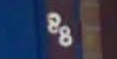
\includegraphics[width=\linewidth]{images/train/1046.png}
\endminipage\hfill
\minipage{0.32\textwidth}
	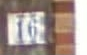
\includegraphics[width=\linewidth]{images/train/10.png}
\endminipage\hfill
\minipage{0.32\textwidth}
	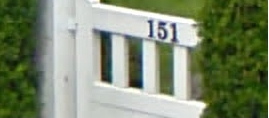
\includegraphics[width=\linewidth]{images/train/20.png}
\endminipage\hfill
\caption{Examples of SVHN imagery from the training set.}
\label{fig:example_imagery}
\end{figure}

\begin{figure}
\minipage{0.32\textwidth}
	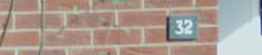
\includegraphics[width=\linewidth]{images/test/37.png}
\endminipage\hfill
\minipage{0.32\textwidth}
	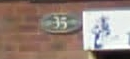
\includegraphics[width=\linewidth]{images/test/38.png}
\endminipage\hfill
\minipage{0.32\textwidth}
	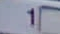
\includegraphics[width=\linewidth]{images/test/39.png}
\endminipage\hfill
\caption{Examples of SVHN imagery from the testing set.}
\label{fig:example_test_imagery}
\end{figure}

\begin{figure}
\minipage{0.32\textwidth}
	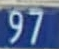
\includegraphics[width=\linewidth]{images/extra/140.png}
\endminipage\hfill
\minipage{0.32\textwidth}
	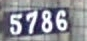
\includegraphics[width=\linewidth]{images/extra/148.png}
\endminipage\hfill
\minipage{0.32\textwidth}
	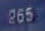
\includegraphics[width=\linewidth]{images/extra/156.png}
\endminipage\hfill
\caption{Examples of SVHN imagery from the extra set.}
\label{fig:example_extra_imagery}
\end{figure}

Figures \ref{fig:example_imagery} and \ref{fig:example_test_imagery} demonstrate some examples of the kinds of imagery we are dealing with in the SVHN dataset for training and testing. 
As you can see, there is a lot of variability in both the image size and image quality. 
For example in the center image, we can just barely tell that the first digit is a 1, but it could easily be misconstrued as a 7. 
However, one advantage that is provided by this data set is that digits, while not necessarily front and center, are at least prominent within the image.

Another potential complication is demonstrated by the left-most image, which shows that not all of the individual digits are lined up nicely.
Some of them are stacked diagonally or even vertically, and the neural network must be able to figure this out.

Many of these images are of relatively low quality, and present a considerable challenge to the neural network to learn.
However, as you can see from Figure \ref{fig:example_extra_imagery}, the imagery from the Extra data set is of considerably higher quality.
The digits are far less blurry, and tend to already take up the majority of the image.
This makes them much easier to work with because we will need far less resizing to bring the digits to the forefront of the image.

\subsection{Exploratory Visualization}
The first interesting property about the SVHN data set is the distribution of digit lengths across the different partitions (training, testing and extra).
Each image has one to five digits in the house number.
However, as shown in Figures \ref{fig:digit_length_plots} and \ref{fig:digit_length_table}, the digit lengths are not all equally represented by the training data.
This is likely representative of the relative probability of seeing a house number of each given length, but also raises the potential for the model to learn a bias towards common digit lengths, or against those less common ones.
As the data shows, digit lengths of two and three are far more common, while five digit house numbers are almost non-existent.

\begin{figure}[!htb]
\centering
\subfloat[Training\label{fig:train_digit_length_plot}]{
	\centering
	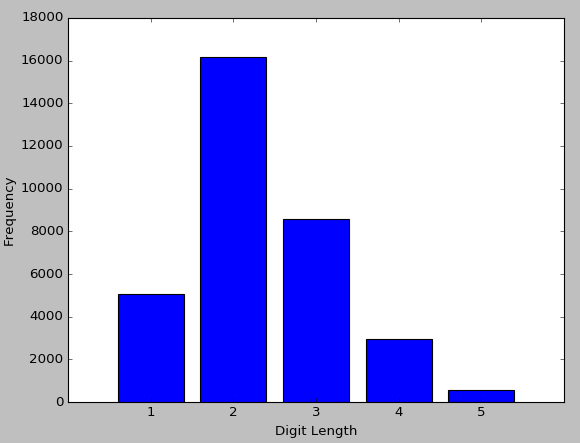
\includegraphics[width=0.45\columnwidth]{images/results/train_digit_lengths.png}
}\hfill
\subfloat[Testing\label{fig:test_digit_length_plot}]{
	\centering
	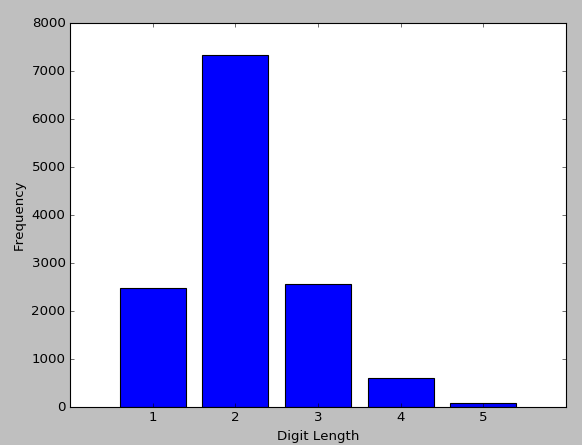
\includegraphics[width=0.45\columnwidth]{images/results/test_digit_lengths.png}
}\hfill
\subfloat[Extra\label{fig:extra_digit_length_plot}]{
	\centering
	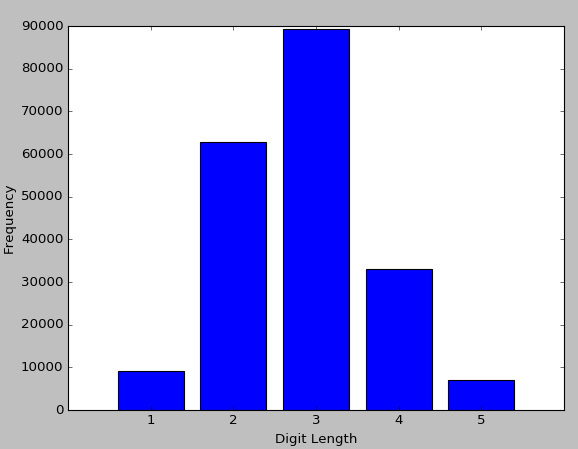
\includegraphics[width=0.45\columnwidth]{images/results/extra_digit_lengths.png}
}\hfill
\caption{Distributions of digit lengths for each of the training sets.}
\label{fig:digit_length_plots}
\end{figure}

\begin{figure}[!htb]
\begin{center}
\begin{tabular}{ |c|c|c|c|c|c| }
\hline
       & 1       & 2       & 3       & 4       & 5       \\
\hline
Train  & 15.25\% & 48.48\% & 25.69\% & 8.86\%  & 1.72\%  \\
\hline
Test   & 18.94\% & 56.13\% & 19.56\% & 4.67\%  & 0.70\%  \\
\hline
Extra  & 4.52\%  & 31.19\% & 44.36\% & 16.43\% & 3.48\%  \\
\hline
\end{tabular}
\end{center}
\caption{Ratio of each digit length's presence in its respective data set.}
\label{fig:digit_length_table}
\end{figure}

\begin{figure}[!htb]
\centering
\subfloat[Training\label{fig:train_digit_freq_plot}]{
	\centering
	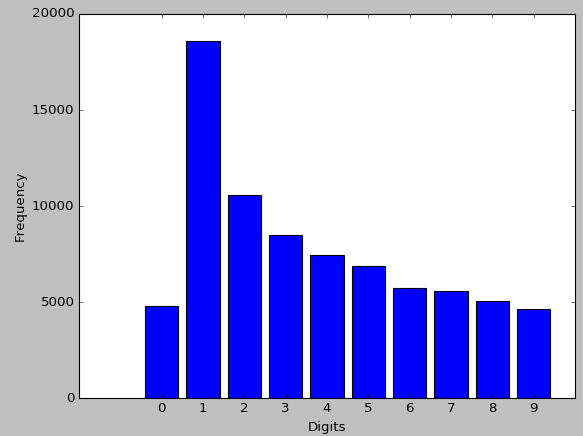
\includegraphics[width=0.45\columnwidth]{images/results/train_digit_freq.png}
}\hfill
\subfloat[Testing\label{fig:test_digit_freq_plot}]{
	\centering
	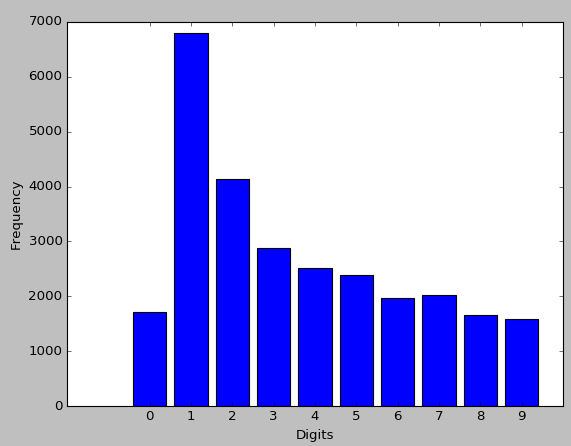
\includegraphics[width=0.45\columnwidth]{images/results/test_digit_freq.png}
}\hfill
\subfloat[Extra\label{fig:extra_digit_freq_plot}]{
	\centering
	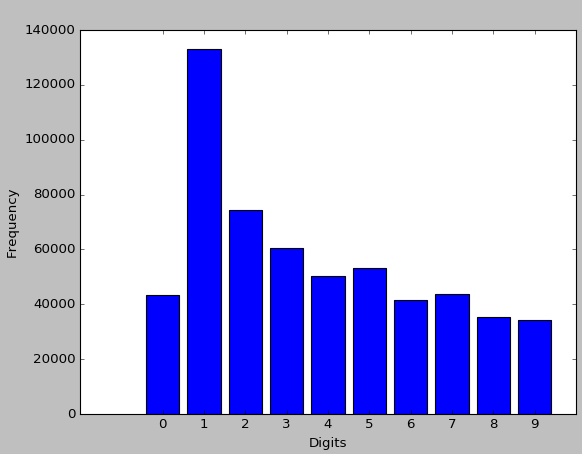
\includegraphics[width=0.45\columnwidth]{images/results/extra_digit_freq.png}
}\hfill
\caption{Distributions of individual digit frequencies for each of the training sets.}
\label{fig:digit_freq_plots}
\end{figure}

There is a similar asymmetry with the distribution of the individual digits.
As demonstrated by Figure \ref{fig:digit_freq_plots}, the digit 1 is by far the most common digit across all data sets.
Similar to the digit length bias, this asymmetry creates a potential bias towards the digit 1 in the model's predictions.
Even if there is not a bias, the model may be far more successful in recognizing 1's relative to other digits.

\subsection{Algorithms and Techniques} \label{sssec:algs}
In order to solve this problem, a convolutional neural network has been employed.
Convolutional neural networks are currently the most successful model employed for most computer vision problems.
For classification tasks, neural networks output a probability distribution representing their confidence in each class.
The prediction of the network is chosen as the label with the highest confidence probability score.

Neural networks do not inherently emit probabilities.
The outputs of neural networks are fundamentally just weighted sums of the input values passed through a non-linear function, the combination of which is not guaranteed to sum to 1.
An additional technique (layer) is required to achieve this effect, the most common of which (and the one used in this project) is the \textit{softmax} function.
This technique essentially uses proportional representation to scale all of the values of a vector in $\mathbb{R}^n$ such that they sum to 1.
It is defined element-wise as follows:

\begin{equation}
	S(x)_j = \frac{\exp(x_j)}{\sum_{i=1}^{n} \exp(x_i)}
\end{equation}

Overfitting was combatted by using a technique called \textit{dropout}\cite{svhn_dropout}.
Dropout layers will randomly set the output of a neuron to 0 (at training time only).
This has the effect of forcing the neural network to learn alternate representations of the input data.
This is because it cannot depend upon any particular representation being consistently correct during the training process.

Another technique used to help prevent overfitting is \textit{max pooling}.
Max pooling is the process of down-sampling the image by taking the maximum pixel value within square grid areas across the entire image.
For example \footnote{Image courtesy of http://cs231n.github.io/convolutional-networks/}:

\hfill \break
\begin{centering}
	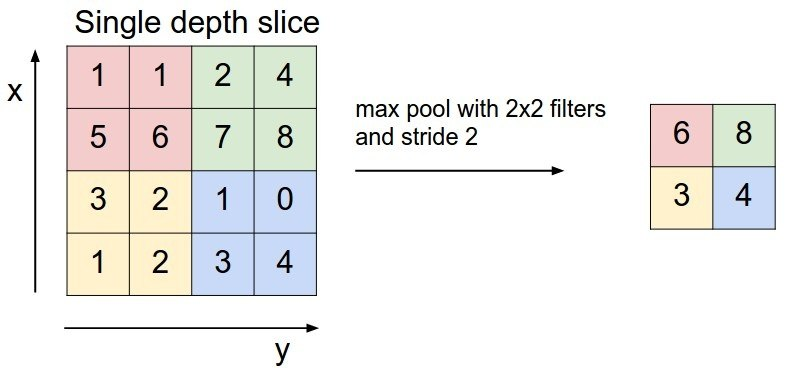
\includegraphics[width=0.85\columnwidth]{images/maxpool.jpg}
	\label{Testing}
\end{centering}
\hfill \break

Max pooling reduces overfitting by gradually reducing the number of parameters in the model.
This also has the added benefit of reducing computational complexity. 

Initialization of the weights in the network was done using Xavier initialization \cite{xavier}.
Xavier initialization is a technique for controlling the variance of the inputs and outputs of a layer of neurons, aiming to keep them more or less the same.
If these variances are not controlled, then it would be possible for the gradiants passing through the network to either vanish or grow exponentially, making the network useless. 
This effect would depend on the size of the network, as well as what the initial values are set to.
By controlling the variances, we are ensuring that the weights stay within a consistent range of values across all layers in the network, allowing the gradiants emitted from one layer to be sensible when processed by the next.

For this project, I have used an architecture similar to the one described in the original paper \cite{svhn_original_paper}, which means that we will have a unique softmax classifier for each digit in the house number.
This does, however, mean that there is a hard limit on the number of digits that can be recognized by the model.
As in the original paper, I have chosen that limit to be five.
One divergence from the original paper is the lack of a length prediction classifier.
In the original paper, if a house number was less than five digits long, then the prediction would have random predictions for the stranded digits.
This was remedied by a sixth classifier output that would provide the digit length, thereby allowing you to determine which digits were true predictions.

While this approach was tested during this project, superior results were achieved by discarding the length prediction and simply introducing a placeholder digit class to signify that the digit does not exist in the picture.

This algorithm contains several hyper-parameters:

\begin{itemize}
	\item The optimization algorithm $\mathcal{O}$ is responsible for using the output of the loss function $\mathcal{L}$ to update the weights of the neural network. Several different algorithms were tested, including Adam, Adagrad and Adadelta. $\mathcal{O}$ also has several hyper-parameters of its own:
	\begin{itemize}
	\item While the optimizer $\mathcal{O}$ determines the relative distribution of the updates to the weights in the network, the learning rate $\alpha$ determines how large those updates end up being.
	\item The use of exponential decay introduces several other parameters: the initial learning rate $\alpha_0$, the number of epochs $\varepsilon$ over which the decay takes place, and the final learning rate $\alpha_{\varepsilon-1}$.
	\end{itemize}

	\item The neural network architecture:
	\begin{itemize}
		\item The number of layers in the neural network. This has a direct impact on the number of parameters used in the model.
		\item The number of filters in each convolutional layer.
		\item The receptive field size in each convolutional layer.
		\item The stride and padding of the convolutional layers.
		\item The size of the fully connected layers (in terms of units).
		\item The training dropout rate.
		\item The stride and padding of the max-pooling layers.
	\end{itemize}

	\item Input normalization parameters:
	\begin{itemize}
		\item The use of statistical centering techniques, such as mean subtraction or variance normalization.
		\item Input image size.
	\end{itemize}
\end{itemize}

Once loaded and normalized, the training data is randomly sampled in batches of 64 and run through the neural network and its optimizer.
Backpropagation of the loss $\mathcal{L}$ is done using the Adagrad optimizer.

Every 100 iterations the validation set is run through the network and its accuracy measured and recorded.
If the performance on the validation set is the best seen thus far, then  the model is checkpointed to disk so that it can be restored later and used in production.
This process continues until no improvement is observed for several hours (no hard limit was set).
The best performing model (according to the performance on the validation set) is then used for testing and production.

All training and testing was done on a GPU using TensorFlow version 0.10.


\subsection{Benchmark}
The primary benchmark used for this project was from the original paper \cite{svhn_original_paper}, where they cite 96\% accuracy on the SVHN data set. As this is my first deep learning project, I set the goal of achieving over 85\% accuracy on the testing set.

\section{Methodology}
\subsection{Data Preprocessing}
Upon initialization of the training algorithm, the training data is loaded from disk into memory.
The data is then split into training and validation sets.
The split is performed by first randomly shuffling the data, and then randomly sampling 2,000 examples and setting them aside as the validation set.

Following this step, the images are cropped based on the bounding boxes from the training file (CSV) and then resized to a $32 \times 32 \times 3$ NumPy array.
The images are cropped in order to make sure the digits are front and centre.
This helps the learning algorithm identify the digits better by reducing the amount of noise it has to deal with.
In reality we would not be dealing with such convenient imagery, but this step is used as a placeholder for localization techniques that are beyond the scope of this project.

Following the cropping step, the mean $\mu_t$ of all of the pixels in all of the training images (not from the validation set) is computed and stored to disk. 
$\mu_t$ is then subtracted element-wise from all of the pixels in the training and validation sets as a normalization step.
The training mean is stored to disk because it must also be subtracted from any images we run as part of the testing or in production, since the model will be trained with such a normalization in mind.

\subsection{Implementation}
All applications created for this project were written in Python2 using TensorFlow, NumPy, and SciPy. 
They were developed on a Linux desktop, and training was performed on a GTX 1080 GPU.
All applications were written as command line applications.
Development was done using the PyCharm IDE.

The core of the project is in the convolutional neural network training application.
The first step of this application is in loading and preparing the training data.
The data is loaded baseed on the parameters provided at the command line. 
The training data is expected to all be contained within a folder that contains the images and the CSV file providing the labels and bounding boxes.

The CSV file contains all of the filenames of the images, and hence is loaded first.
Once the CSV file is loaded the entries are shuffled, and 2,000 entries are randomly sampled and removed from the training set.
These are reserved for validation and will not be used for training.

When each image is loaded, its corresponding CSV entry is simultaneously loaded, and the resizing and cropping is performed at that time.
All image loading and manipulation techniques are performed using SciPy, and the final image is stored as a NumPy array.
After the image has been cropped and resized, the bounding boxes are discarded, and only the labels and images are kept in memory.
The final result of this operation is two lists of equal size: The first containing all of the images, and the other containing all of the labels. They are returned as a 2-tuple from the image loading sub-routine.

This process can be fairly CPU-intensive, and I found that while using the extra data set as training, the loading time would take several minutes. 
Therefore, the data loading algorithm was augmented to use Python's multiprocessing library.
Now the algorithm will use all available (logical) CPUs to perform the data import.
Now the loading time (on my home computer) takes only a few seconds instead of over three minutes.

The final step in the data loading process is to compute the mean pixel value $\mu_t$ across all of the images in the data set.
This value is subsequently subtracted from each image as a normalization step.
Furthermore, since this mean would need to be subtracted from images processed during the test or production phases, the value is written out to a text file in the output folder.

The next step is to construct the computational graph.
This is done using raw TensorFlow.
Initially Keras was used to create the graph, but I found it to be limited when it came to constructing networks with multiple outputs.

Before the training process begins, a model Saver is created targeting the output directory (provided at the command line).
Training samples are provided to the graph in batches that are randomly sampled from the training set.
Furthermore, every 100 iterations the entire validation set is run (as a single batch) and its accuracy computed.
If the accuracy of the validation set is the best seen so far, then the model is checkpointed to the output directory.
I also keep a record of all of the training and validation accuracies (as well as the training loss) every 100 iterations, which are written to a CSV file in the output directory.
This CSV file is used by another Python application I wrote that generates PyPlot graphs that summarize the performance of the training algorithm over time.

There are two other applications that load the data that is output by the training program.
The first is an application that is solely responsible for running tests against a labelled data set.
It uses all of the same data loading techniques as the training program, but it loads the model from disk (the output of the training program) and does not perform any of the back-propagation. 
Instead, it simply tallies the accuracies from all of the testing batches and outputs the result.

The second application is meant to be used in production.
It is invoked on the command line and consumes a batch of unlabelled images and produces a CSV file with the predictions for each file.
This application uses a slightly simpler data loading algorithm.
It has no bounding boxes, therefore it only resizes the image instead of cropping it. 
It does, however, have access to the training mean file that was produced by the training program, therefore it is able to perform normalization on the input images.

\subsection{Refinement}
The largest sources of improvement during this project were the adjustment of the learning rate and increasing the size of the network.

The initial network consisted of four convolutional layers and one fully connected layer which then lead to five output layers.
The convolutional layers had depths of 48, 64, 128 and 160.
The fully connected layer consisted of 2048 units.
This was followed by five softmax classifiers (one for each digit) as the output layers.
Max pooling was used after the second and fourth convolutional layers, reducing the image by half each time.
Dropout was also used on the first and third convolutional layers, as well as the fully connected layer, each time with a dropout probability of 50\%.
The convolutional layers each used $5 \times 5$ receptive fields with a stride of 1.
All weights were initialized using Xavier initialization \cite{xavier}.

The learning rate was initially set statically to 0.05.
This allowed the accuracy to reach 80\%, however once it reached this point, the network would suddenly jump out of its current optimum, and land somewhere completely sub-optimal. 
This can be seen in Figure \ref{fig:small_network_results}.
Whether this was a Tensorflow bug, or as a result of a flawed architecture, was not discernable.
However, I suspect that the learning rate was the real culprit.
Such a learning rate was clearly too high to allow the optimizer to find the smaller crevices of the cost function that lead to higher accuracies.

In response to this the learning rate was lowered to 0.025, and set to exponentially decay to 0.001.
Furthermore, the size of the network was doubled to its final form, which is outlined in detail in Section \ref{sssec:evaluation}.
With these changes, the accuracy (on the validation set) was able to exceed 90\%. 
Those results are discussed in Section \ref{sssec:justification}.

Adding additional layers obviously increases the size of the model and allows it to learn a greater variety of features.
However, I observed the biggest gain in performance by adjusting the learning rate and introducing exponential decay.
As previously discussed, lowering the learning rate would allow it to navigate to smaller crevices of the cost function.
However, there is some utility in allowing a larger learning rate at the beginning of the learning process. 
At the beginning of the process, the model is more or less randomly initialized.
This means that the model is likely to be nowhere near the optimal solution.
A larger initial learning rate would therefore allow it to more quickly navigate to the general vicinity of the optimal solution.
Once the model has reached such a region, then it makes intuitive sense to start lowering the learning rate, as the steps required to improve become increasingly nuanced.
Keeping a large learning rate could cause the optimizer to overshoot the narrower valleys in the cost function.
In theory, such a high learning rate could actually cause the optimizer to \textit{diverge}, as the momentum of such a high learning rate could expell the model from a valley in the cost function.
I suspect that this is a possible cause of the phenomena observed in Figure \ref{fig:small_network_results}, and hence why performance not only improved with a smaller learning rate, but became more stable.

There were two approaches attempted with the final architecture.
The most successful of which has been outlined in Section \ref{sssec:evaluation}.
The second method was the one described in the original paper \cite{svhn_original_paper}, which uses length prediction instead of placeholder digits.
The length prediction method was attempted and achieved a 90.1\% validation accuracy, which is shown in Figure \ref{fig:length_best_results}.
This result was impressive, but the result of 96\% using placeholder digits easily eclipsed it.
The results of that run are demonstrated in Figure \ref{fig:final_moredata}.

\begin{figure}[!htb]
\centering
\subfloat[Loss\label{fig:lenth_best_loss}]{
	\centering
	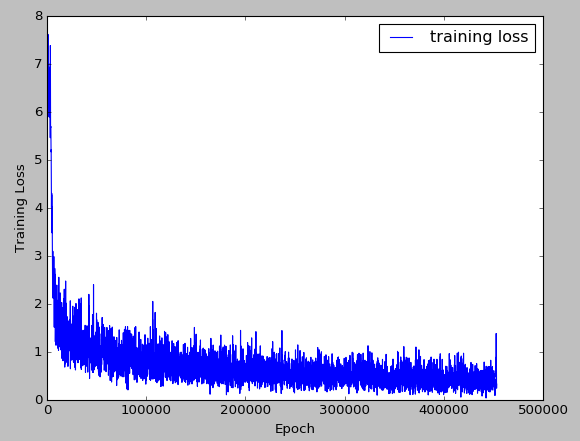
\includegraphics[width=0.45\columnwidth]{images/results/length_best_loss.png}
}\hfill
\subfloat[Accuracy\label{fig:length_best_accuracy}]{
	\centering
	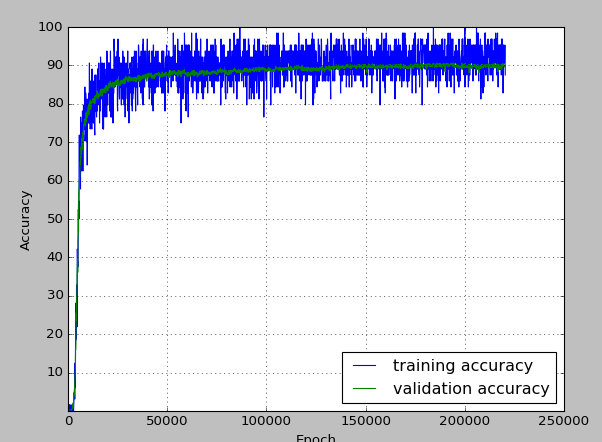
\includegraphics[width=0.45\columnwidth]{images/results/best_accuracy.png}
}\hfill
\caption{Plot of best run using length prediction, $\alpha_0 = 0.025$, 50,000 epoch decay to 0.0075.}
\label{fig:length_best_results}
\end{figure}

\begin{figure}[!htb]
\centering
\subfloat[Loss\label{fig:small_best_loss}]{
	\centering
	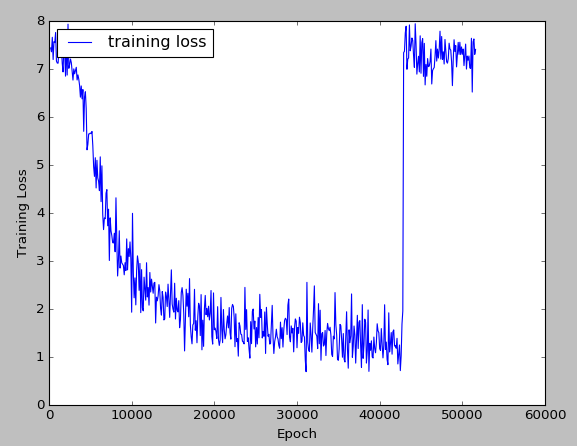
\includegraphics[width=0.45\columnwidth]{images/results/small_network_loss.png}
}\hfill
\subfloat[Accuracy\label{fig:small_best_accuracy}]{
	\centering
	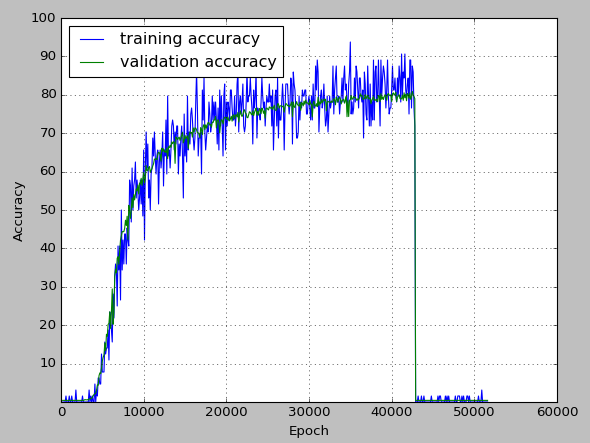
\includegraphics[width=0.45\columnwidth]{images/results/small_network_accuracy.png}
}\hfill
\caption{Plot of run using smaller convolutional network, $\alpha_0 = 0.025$, 30,000 epoch decay to 0.001.}
\label{fig:small_network_results}
\end{figure}

\section{Results}
\subsection{Model Evaluation and Validation} \label{sssec:evaluation}
The final architecture of the neural network is roughly based on the design outlined in the original paper \cite{svhn_original_paper}.
The network uses eight convolutional layers, with depths of 48, 64, 128 and 160 for the first four layers, and 192 for the final four layers.
This is followed by two fully connected layers with 4096 units each.
The network then splits into five output layers, each one predicting one of the up-to-five digits in the image. 
Each output layer is assigned a static index $i$, and that layer is responsible for predicting the $i$-th digit. 
If the number has fewer digits than $i$, then the output layer will output the null class, which in this case is just the digit 10.
Each output layer is a fully connected softmax classifier.

Every convolutional layer and pre-output fully connected layer uses ReLU\cite{relu} activations followed by dropout\cite{svhn_dropout} and local response normalization\cite{svhn_lrn} layers.
The convolutional kernel size for all convolutional layers was $5 \times 5$, along with a stride of 1.

Max pooling was used twice, once following convolutional layer 4, and again following convolutional layer 8.
Both max pooling layers used $2 \times 2$ windows with a stride of 2.

The Adagrad optimizer was used with exponential decay. I used an initial learning rate $\alpha_0 = 0.025$, decaying over the course of 50,000 epochs to a final learning rate of 0.001.

\subsection{Justification} \label{sssec:justification}
For this evaluation, two different models were used.
For the first model, only the training set was used for training, and achieved a validation accuracy of 89.9\% and a testing accuracy of 82.7\%, which falls short of the 85\% goal I set for myself.
These results are shown in Figure \ref{fig:final_lessdata}.
However, the same model's accuracy when testing on the extra data set (which was not used for any kind of training) achieved 95.8\% accuracy.
The second model used both the training and extra sets for training, and achieved a validation accuracy of 96\% and a testing accuracy of 88.8\% on the testing set.
These results are shown in Figure \ref{fig:final_moredata}.

Additional testing was performed on a custom data set that was collected from the internet, as well as from my own neighborhood.
These results are called the \textit{custom} data set, and can be found in the uploaded data \footnote{All project data can be found \href{https://drive.google.com/open?id=0B918sU9DDf8DTElNWGhwN1pTTXM}{here}.}.
What these experiments made clear was that there is one major weakness in the approach taken for this project.
That weakness is that the algorithm has a very fragile sense of localization.
The algorithm performed very poorly on any imagery that was not cropped such that the digits were front and center.
If the digits were not the prominent elements in the image, then the output is completely incorrect.
However, if appropriate cropping is performed, then performance improves dramatically, and comes in line with the observed results from the training and validation sets.
These results are visualized in Section \ref{sssec:ffv}, and potential solutions to the aforementioned shortcomings are discussed in Section \ref{sssec:improvement}.

\begin{figure}
\centering
\subfloat[Loss\label{fig:final_loss_lessdata}]{
	\centering
	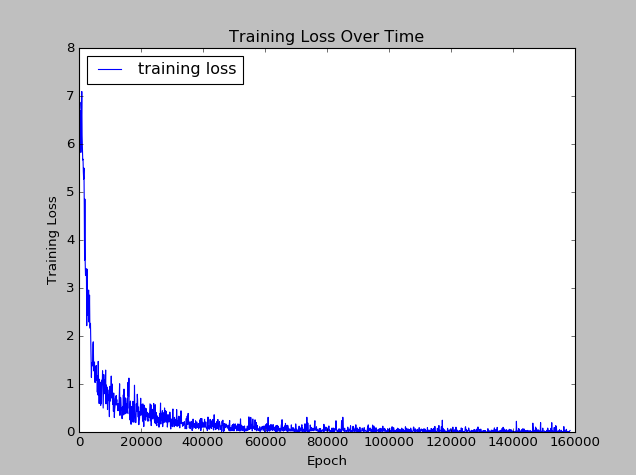
\includegraphics[width=0.45\columnwidth]{images/results/train_loss_lessdata.png}
}\hfill
\subfloat[Accuracy\label{fig:final_accuracy_lessdata}]{
	\centering
	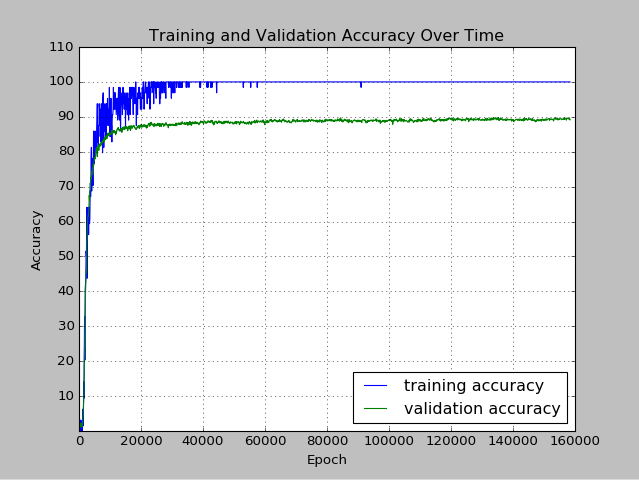
\includegraphics[width=0.45\columnwidth]{images/results/accuracy_lessdata.png}
}\hfill
\caption{Plot of run using larger convolutional network, $\alpha_0 = 0.025$, 50,000 epoch decay to 0.001. Trained using just the training set.}
\label{fig:final_lessdata}
\end{figure}

\begin{figure}
\centering
\subfloat[Loss\label{fig:final_loss_moredata}]{
	\centering
	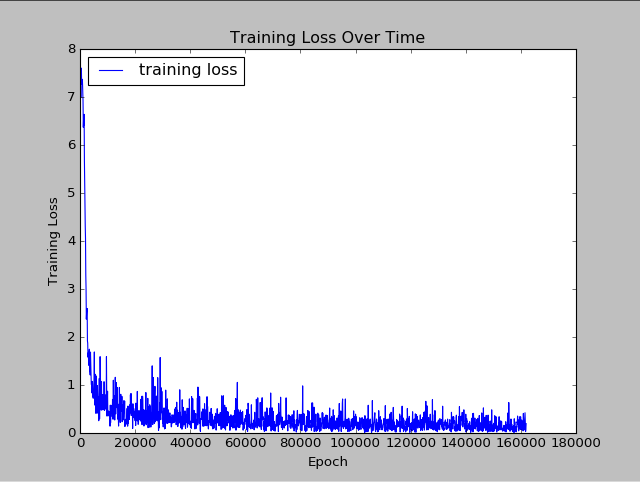
\includegraphics[width=0.45\columnwidth]{images/results/training_loss_moredata.png}
}\hfill
\subfloat[Accuracy\label{fig:final_accuracy_moredata}]{
	\centering
	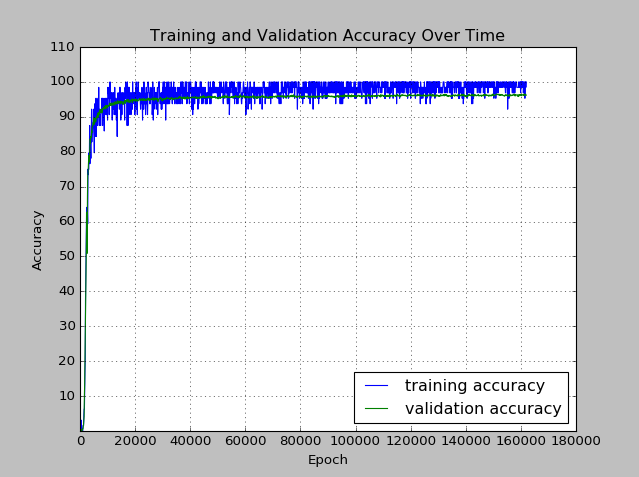
\includegraphics[width=0.45\columnwidth]{images/results/accuracy_moredata.png}
}\hfill
\caption{Plot of run using larger convolutional network, $\alpha_0 = 0.025$, 50,000 epoch decay to 0.001. Trained using the union of training and extra sets.}
\label{fig:final_moredata}
\end{figure}

\section{Conclusion}
\subsection{Free-Form Visualization} \label{sssec:ffv}
Figure \ref{fig:custom_visualizations} demonstrates some of the weaknesses of this algorithm.
The results of the first pair of images are not altogether surprising.
The algorithm was not trained to evaluate text, and therefore it is not surprising that text confuses the algorithm.

The remaining images demonstrate the algorithm's utter inability to cope with external objects. 
Even in the cropped image, we can see that it made an error. 
I would hypothesize that it got confused by the shadow cast by the 1, and interpreted it as an extra digit.
The root of this problem is likely the cropping of the training data.
The algorithm has not had much of an opportunity to observe noise in the data and thus learn the difference between digits and background objects such as bricks and lamps.

\begin{figure}[!htb]
\centering
\subfloat[Original image. Predicted label: 32.\label{fig:custom1}] {
	\centering
	
\includegraphics[width=0.45\columnwidth]{images/custom/2.jpg}
}\hfill
\subfloat[Cropped image. Predicted label: 2\label{fig:custom1_cropped}] {
	\centering
	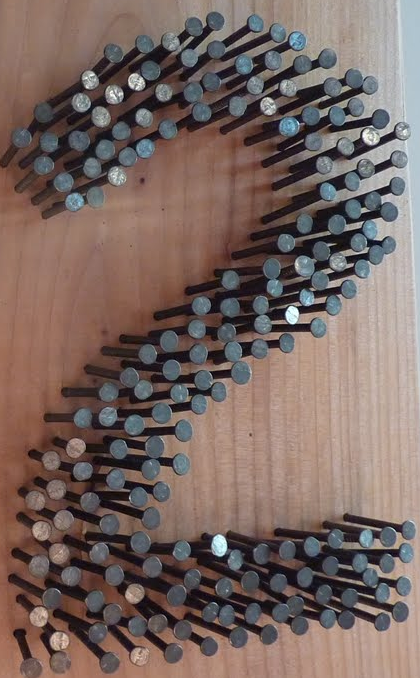
\includegraphics[scale=0.25]{images/custom/2-cropped.png}
}\hfill

\subfloat[Original image. Predicted label: 266.\label{fig:custom2}] {
	\centering
	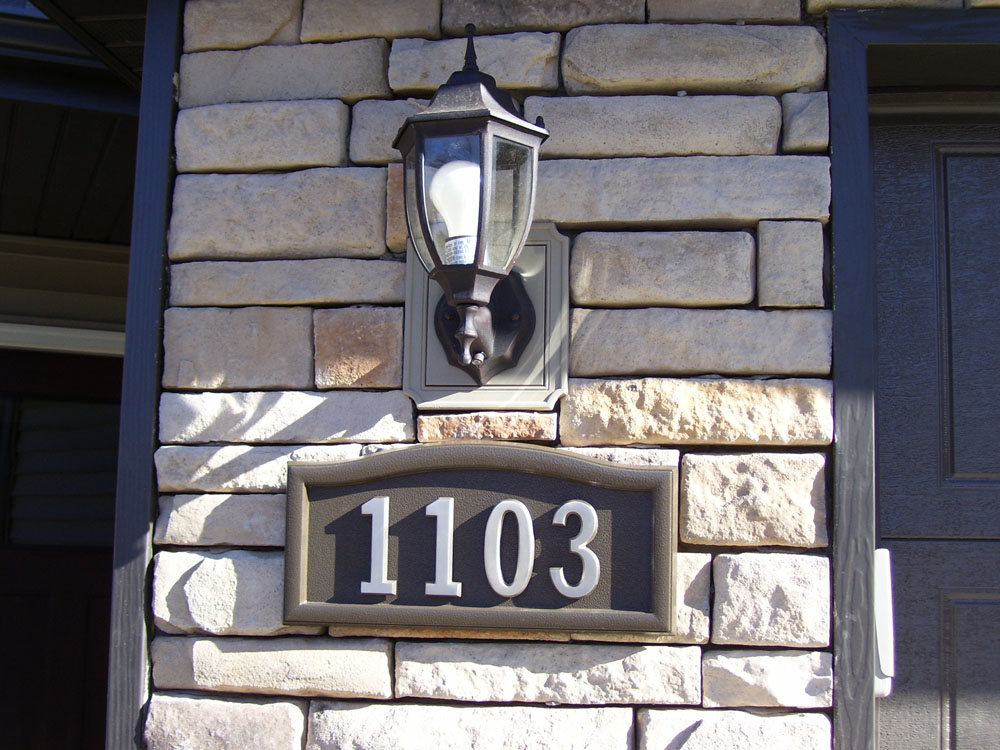
\includegraphics[width=0.45\columnwidth]{images/custom/1103.jpg}
}\hfill
\subfloat[Cropped image. Predicted label: 11103.\label{fig:custom2_cropped}] {
	\centering
	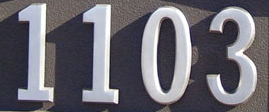
\includegraphics[scale=0.60]{images/custom/1103-cropped.png}
}\hfill

\subfloat[Original image. Predicted label: 188.\label{fig:custom3}] {
	\centering
	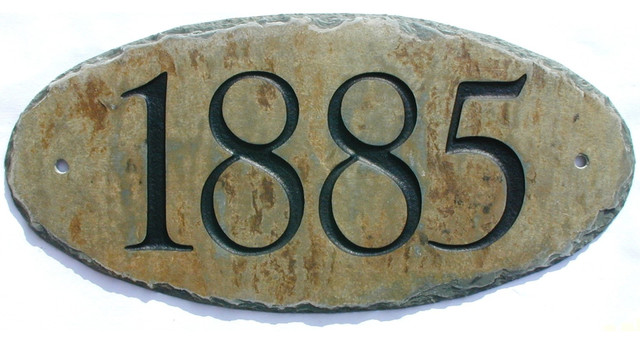
\includegraphics[width=0.45\columnwidth]{images/custom/1885.jpg}
}\hfill
\subfloat[Cropped image. Predicted label: 1885.\label{fig:custom3_cropped}] {
	\centering
	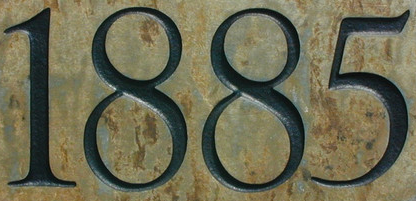
\includegraphics[scale=0.35]{images/custom/1885-cropped.png}
}\hfill

\end{figure}
\clearpage
\begin{figure}[!htb]
\centering
\ContinuedFloat

\subfloat[Original image. Predicted label: 393.\label{fig:custom4}] {
	\centering
	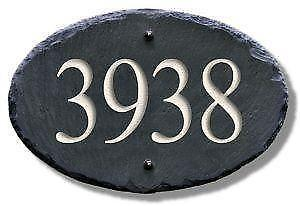
\includegraphics[width=0.45\columnwidth]{images/custom/3938.jpg}
}\hfill
\subfloat[Cropped image. Predicted label: 3938.\label{fig:custom4_cropped}] {
	\centering
	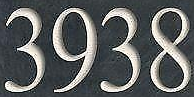
\includegraphics[scale=0.70]{images/custom/3938-cropped.png}
}\hfill

\subfloat[Original image. Predicted label: 472.\label{fig:custom5}] {
	\centering
	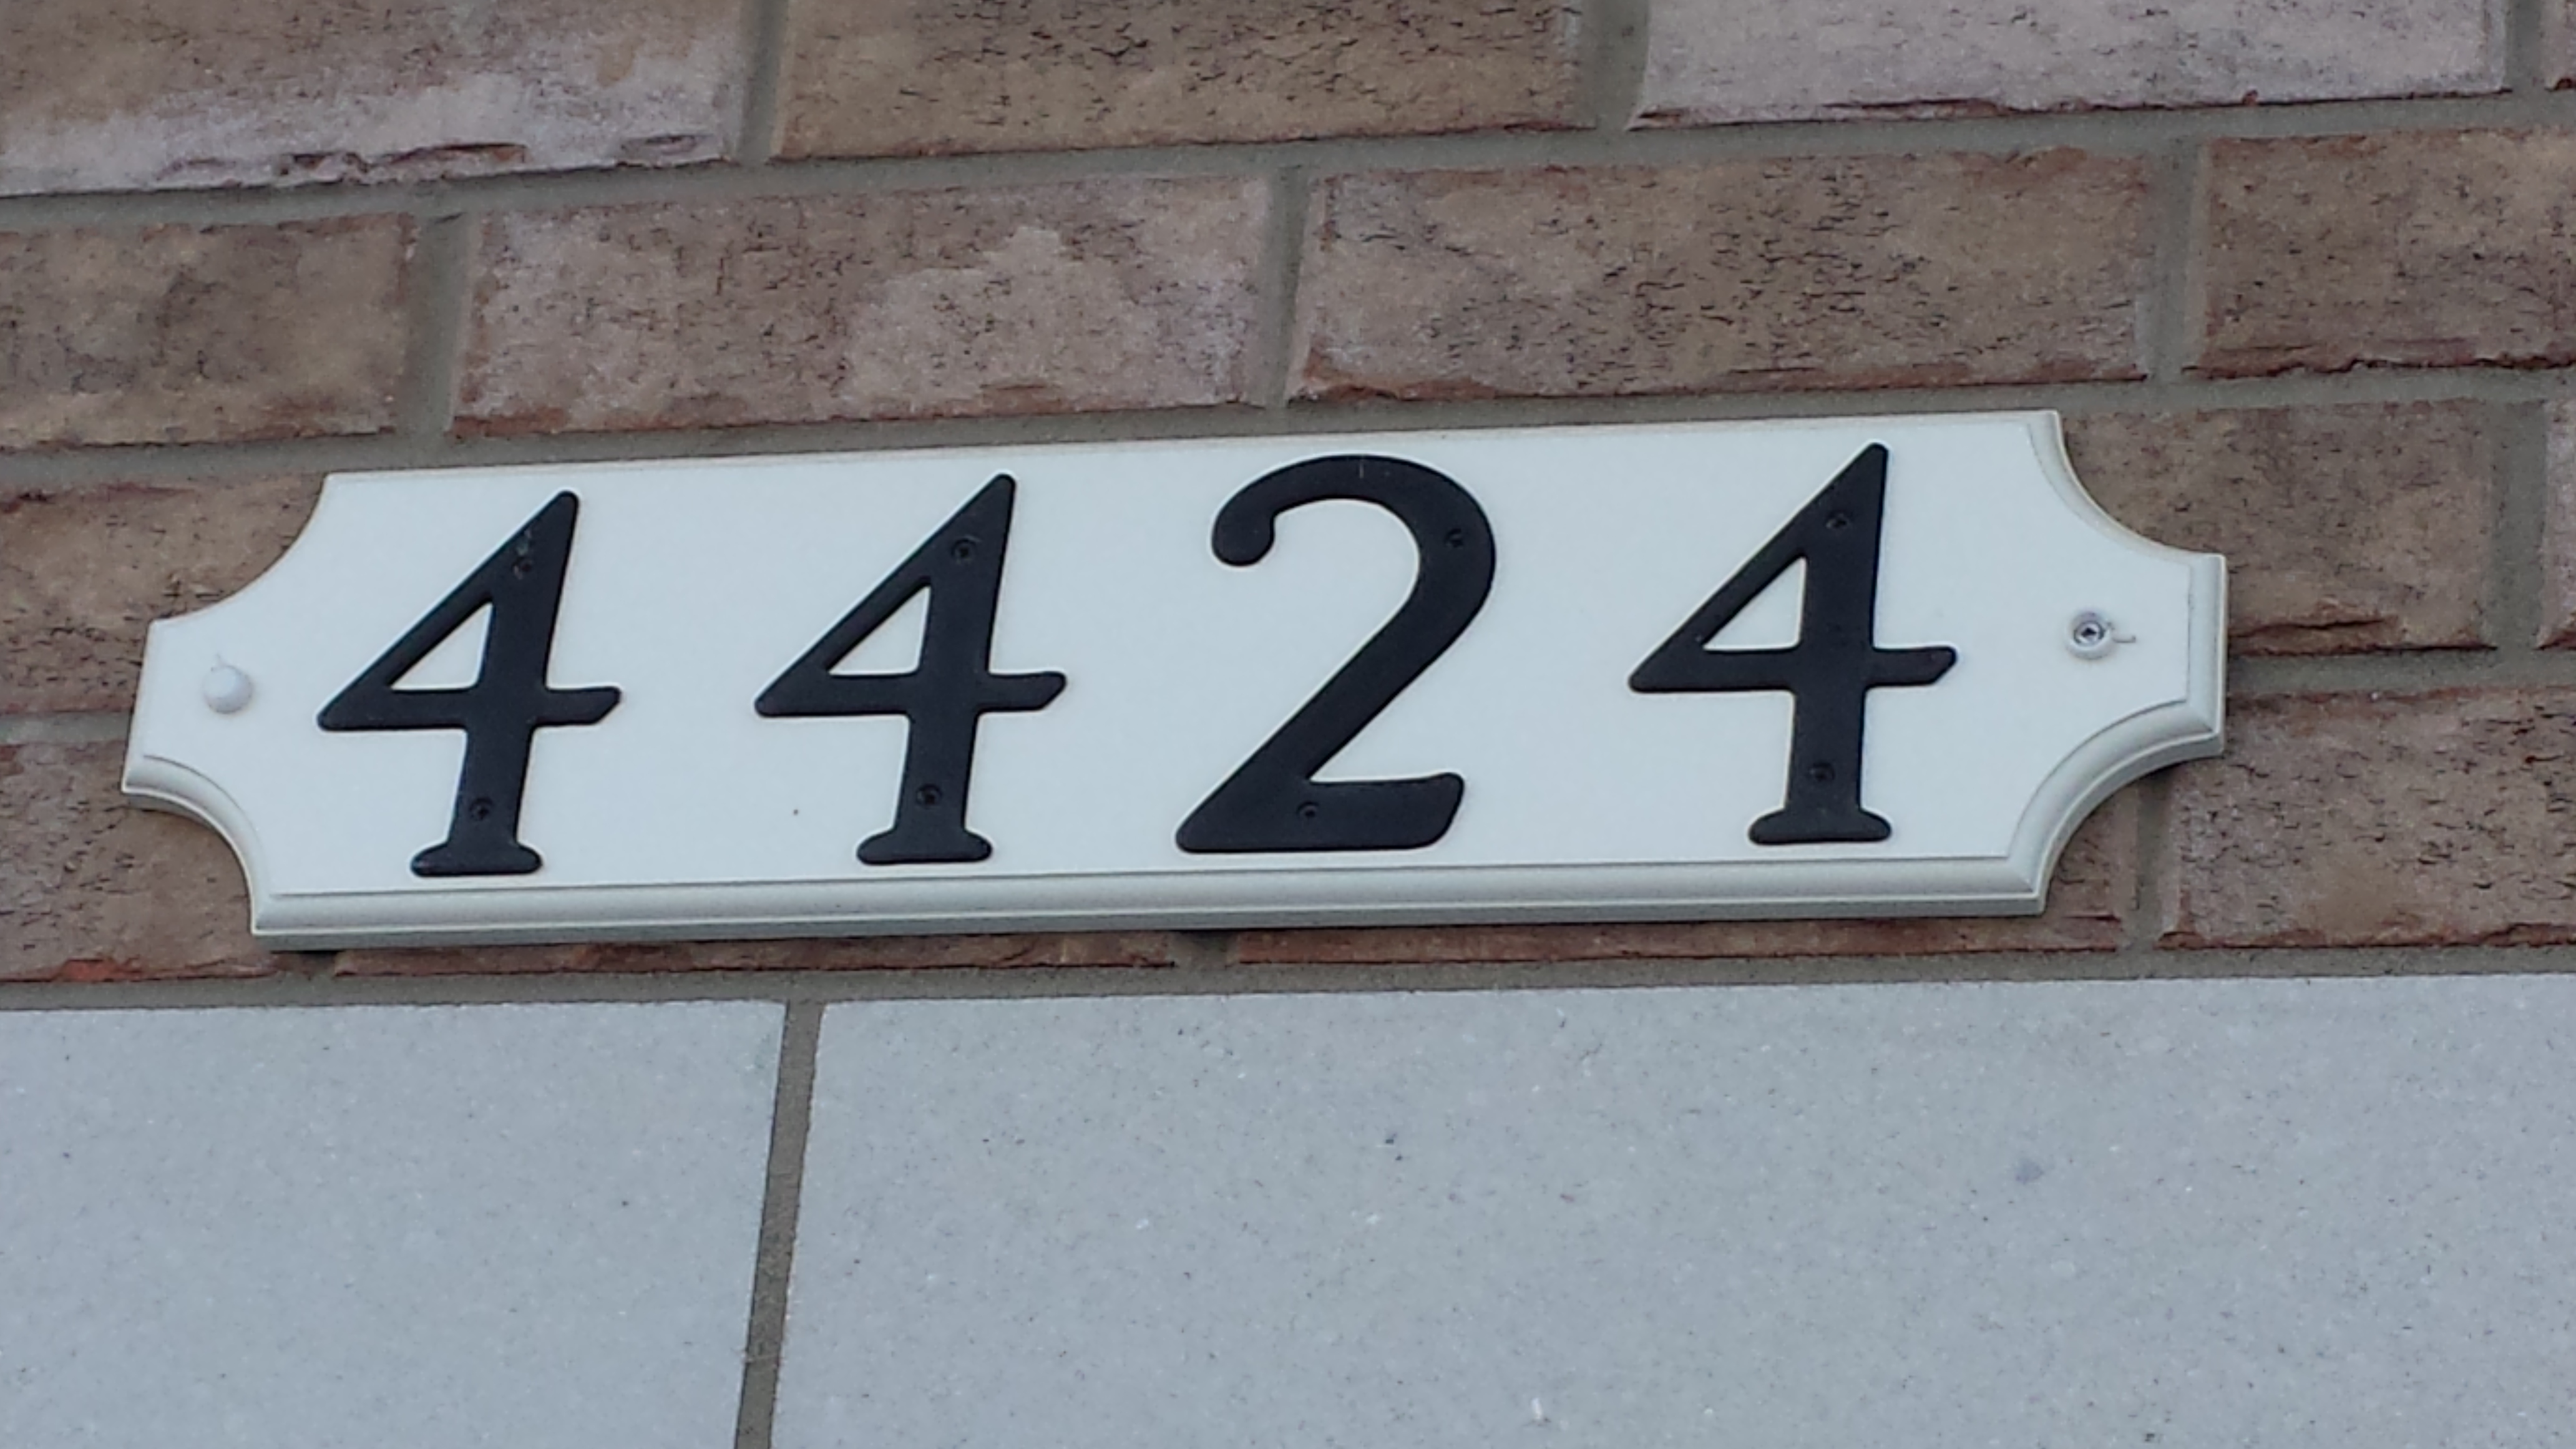
\includegraphics[width=0.45\columnwidth]{images/custom/4424.jpg}
}\hfill
\subfloat[Cropped image. Predicted label: 4424.\label{fig:custom5_cropped}] {
	\centering
	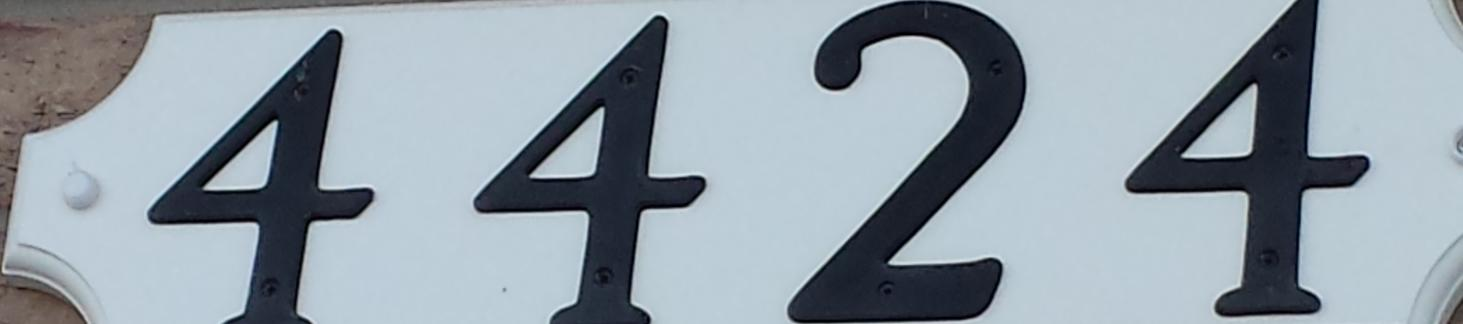
\includegraphics[scale=0.12]{images/custom/4424-cropped.jpg}
}\hfill
\caption{Summary of randomly collected extra imagery. This imagery was used to test how the algorithm generalizes. Each image is presented in its original form, as well as its cropped form, showing the digits prominently in the image.}
\label{fig:custom_visualizations}
\end{figure}

\subsection{Reflection} \label{sssec:reflection}
The steps taken to complete this project are as follows:

\begin{enumerate}
\item The problem was studied, including existing implementations outlined in the original papers \cite{svhn_original_paper,svhn_lrn}.
\item The data set used in the original papers was downloaded and analyzed.
\item Experiments were run in loading, resizing and enhancing the imagery. 
\item The SVHN data set comes in an HD5 file set, which I found to be extremely slow to load and manipulate. Therefore, as the next step, I wrote an application that loads the HD5 files and exports their contents (labels, bounding boxes, etc.) to a CSV format. This was vastly more effecient in terms of loading times.
\item To aid in the analysis, an application was written to load the data from the CSV files and generate various charts and graphs using pyplot. Those visualizations are shown in Section \ref{sssec:algs}.
\item An application was written to do the convolutional neural network training. This is where the majority of the time was spent on this project. This application would load the training data and use it to train the network. The training and validation accuracy was recorded and used as a guide for how to checkpoint the model.
\item In order to test how the model performs on unseen (but still labelled) data sets, another application was written that would load data with labels and run the model against it. This application would calculate the accuracy using the labels.
\item In order to visualize the results of the training stages, an application was written to construct pyplots from the training outputs. Those visualizations are shown in Section \ref{sssec:justification}.
\item Finally, the batch processing application was written that could consume a data set not containing labels and produce a set of predictions.
\end{enumerate}

The most difficult and interesting part of this project was in training the CNN. 
The first several attempts to create the network yielded very poor results, at or near 0\% accuracy.
This ended up being a combination of flaws in my understanding of the TensorFlow library, as well as flaws in my understanding of how to properly construct a neural network.
The arduous process of getting it to work for the first time was truly educational.

The next most difficult aspect was tuning the various parameters of the network to improve performance.
Experiments often take a fairly long time, and thus required a lot of patience.

\subsection{Improvement} \label{sssec:improvement}
The primary improvement that the algorithm requires is the ability to locate likely positions of digits all by itself.
If the locations of potential digits could be learned, then the algorithm could take sub-samples of the images from those predicted locations and perform the cropping by itself.

This could potentially also solve the issue of the algorithm becoming confused by background noise. 
This is because the training process would not need to use cropped imagery, therefore allowing the algorithm to be exposed to all kinds of background noise.
If the algorithm were to be exposed to extensive background noise, then it would also learn that not everything is a digit, which could potentially address a lot of the issues displayed in Section \ref{sssec:ffv}.

This would also mean that imagery that is input into the system at production time would not need to be cropped.
As it stands, such a requirement completely invalidates the use of the algorithm, because if you need a human to crop the image, you might as well just have them do the classification instead.

Another consequence of introducing localization would be that it might be possible to do away with the 5-digit limit on the classifier.
If all potential locations could be examined, and digits identified, then in theory all digits in the image could be output.
This introduces a new problem, however. And that would be how to order and group the numbers. 
One could imagine another neural network (or even a hand-crafted algorithm) that could be fed the positions of all of the digits, as well as their dimensions, and produce a prediction of whether or not they are in the same group, as well as which order they belong in.
Such a system could identify all digits in abritrarily sized images, as well as being likely able to classify text. 

\begin{thebibliography}{9}
\bibitem{svhn_dataset} 
Yuval Netzer, Tao Wang, Adam Coates, Alessandro Bissacco, Bo Wu, Andrew Y. Ng 
\textit{Reading Digits in Natural Images with Unsupervised Feature Learning NIPS Workshop on Deep Learning and Unsupervised Feature Learning 2011.}
http://ufldl.stanford.edu/housenumbers/
\bibitem{svhn_original_paper}
Goodfellow, Ian J.; Bulatov, Yaroslav; Ibarz, Julian; Arnoud, Sacha; Shet, Vinay
\textit{Multi-digit Number Recognition from Street View Imagery using Deep Convolutional Neural Networks}
\bibitem{svhn_lrn}
Alex Krizhevsky and Sutskever, Ilya and Geoffrey E. Hinton
\textit{ImageNet Classification with Deep Convolutional Neural Networks}
\bibitem{svhn_dropout}
Nitish Srivastava, Geoffrey Hinton, Alex Krizhevsky, Ilya Sutskever, Ruslan Salakhutdinov
\textit{Dropout: A Simple Way to Prevent Neural Networks from Overfitting}
\bibitem{relu}
R Hahnloser, R. Sarpeshkar, M A Mahowald, R. J. Douglas, H.S. Seung (2000). 
\textit{Digital selection and analogue amplification coesist in a cortex-inspired silicon circuit.}
\bibitem{xavier}
Xavier Glorot, Yoshua Bengio
\textit{Understanding the difficulty of training deep feedforward neural networks}

\end{thebibliography}
	
\end{document}

